The matched width calculations in Table~\ref{tab:widths}, the five
specified PDF coupling checkpoints and all nine signed top/antitop width
and counterterm combinations pass their runtime checks. All 101 members
of the prescribed NNPDF4.0 set are installed and hashed. The measurement
regressions use the actual FastJet wrapper. Generator validation includes
pole cancellation, soft/collinear subtraction checks, analytic/MadLoop
decay-virtual comparisons and exclusive-jet partition identities.
Analytic-provider validation requests MadLoop precision of $10^{-10}$
or better before the independent $10^{-8}$ density comparison.
Numerical fixes to sparse-bin accumulation, near-endpoint phase space,
refinement seeding and massive Born-map ordering are regression-tested;
failed or affected legacy attempts retain their original provenance and
are excluded from certified comparisons.

All six on-shell prescriptions have completed initial single-assignment
pilots for both charges. The independent $S-P-D+\mathrm{LO}$ checks have
maximum absolute central-bin residuals 2.986 and 2.976 MC errors for W$^+$
and W$^-$, over 2802 and 2806 nonzero-error bins. These correlated residuals
are not a global goodness-of-fit test or a publication-precision check.
Earlier stable-production branching tests are provisional because a
subsequent audit found repeated refinement streams in the two-round W$^+$
reference. Fresh NLO inclusive normalization remains required.

The independent native associated-current versus factorized-decay LO
comparison at matched fixed scales gives a decayed/expected ratio
$0.9931\pm0.0041$. The maximum absolute scale/PDF conditional residuals
are 1.71/1.79 MC errors. The native result is multiplied by the two
matched top branching densities only; the associated current receives
no extra branching factor. Actual sampling counts and distinct stage
streams are audited. This supports fixed-scale LO normalization, while
the convergence discrepancy between finite linear/current-proposal
samples still precludes an efficiency or full-support convergence claim.

The latest fixed-source W$^+$ S/$\Pi$ controls use the corrected stage
seeding and Born mapping. All four pass the complete histogram, weight,
virtual and batch audits. Their conditional fiducial ratios appear in
Table~\ref{tab:freshpilots}; none resolves a product shift at the specified
precision. Maximum absolute paired inclusive decay-scale residuals are
0.95/1.13 MC errors for all-BW S/$\Pi$ and 0.27/1.25 for on-shell S/$\Pi$.
These paired cancellations do not replace the independent absolute NLO
current normalization or tests of retraining and sparse-tail convergence.

Direct asymmetric decay scales, $\mu_R^t=2m_t$ and
$\mu_R^{\bar t}=m_t/2$, have now been compared with the corresponding
reweighted coordinates in independent on-shell W$^+$ samples. The direct
one-/two-b rate ratios to reweighting are
$0.9621\pm0.0429$ / $1.0120\pm0.0401$ for S and
$0.9993\pm0.0199$ / $0.9996\pm0.0250$ for $\Pi$.
The 36 distinct matching physical scale points give maximum absolute
rate residuals of 1.30 and 1.57 conditional MC errors. Across the six
normalized spectra and their matching scale coordinates, the maximum is
3.03 MC errors; the few entries above three are correlated bin/scale
comparisons, not a global significance. Each new sample passes 768
analytic-virtual comparisons, and its 130 actual stage initializations
are disjoint from the reference and other controls. These results support
asymmetric reweighting at the measured precision; QES cancellation,
direct BW production-scale checks and the central-scale diagnostics remain
in progress.

\paragraph{Matched literature configuration.}
The first W$^+$ LO/P/S reference calculation uses the separate inputs,
selection and fixed scale of Ref.~\cite{Bevilacqua2020}, including NNPDF3.0
and constant total top widths under scale variation. Under that reference's
unexpanded-width convention, the additive numerator reconstructed as
$[S+2g\,\mathrm{LO}]/(1+g)^2$, $g=\Gamma_{t,1}/\Gamma_{t,0}$, gives
$122.9\pm2.9$ ab, compared with the published rounded 123.0 ab.
The higher-statistics production-only prediction is $126.52\pm0.39$ ab
versus 127.0 ab. These conditional joint-batch errors use 410 distinct stage initializations
across the three independently sampled prescriptions. The reconstructed
NWA seven-point envelope is $[114.2,129.4]$ ab, compared with the published
rounded $[114.3,129.3]$ ab.
The P residual is $-1.21$ times our joint MC error; the reference tables
supply no MC errors, so this is not a combined statistical pull.
An independent lower-statistics P run differs by $2.08\pm1.05$ ab;
the largest absolute difference across the common-scale grid is 2.05
conditional MC errors. Both estimates are retained as convergence evidence.
The NWA reconstruction retains the previously audited LO and S samples;
it is not an additional independent strict-NLO calculation.
The completed W$^-$ calculation gives reconstructed NWA
$67.90\pm0.69$ ab versus 68.0 ab and production-only $70.85\pm0.96$ ab
versus 69.8 ab. These conditional joint errors use 282 distinct stage
initializations, with no overlap between prescriptions.
All raw common-scale weights, workers and stage histories are retained.
These matched references do not release the full phenomenological
campaign by themselves.

The inclusive dilepton-$t\bar t$ calibration uses separate NNPDF3.1 NLO
inputs and common fixed numerator scales $\mu=m_t$, with the supplied
total-width coefficients held fixed under variation~\cite{Behring2019}.
The comparison uses the authors' June 2019 normalized-distribution update.
Against the supplied ten-bin $\Delta\phi(\ell^+,\ell^-)/\pi$ curves, the
largest central-bin residuals are 1.65 combined MC errors for
$S({\rm bin})/S({\rm total})$ and 1.60 for its NLO-expanded normalization.
The latter expansion concerns the normalized observable, independently
of the expansion of the top-width denominators.
Our conditional bin errors range from 1.9--5.9\% and 2.8--9.1\%, respectively;
the supplied central-bin MC errors enter in quadrature. Reference
inter-bin covariance is unavailable, so these correlated residuals are
not a global goodness-of-fit test. All 513 LO/S/$\Pi$ training/refinement
initializations are distinct. This establishes pilot-level compatibility;
percent-level shape precision and retraining coverage remain unverified.
Direct scale/QES and absolute-normalization checks are in progress.

\begin{table}[ht]
\centering
\begin{tabular}{llcc}
\toprule
W treatment & Decay $m_b$ & $\Pi/S$, one-b & $\Pi/S$, two-b\\
\midrule
On shell & $0$ & $0.982\pm0.043$ & $0.993\pm0.037$\\
On shell & $4.8\GeV$ & $1.019\pm0.028$ & $1.000\pm0.032$\\
All BW & $0$ & $1.025\pm0.039$ & $0.939\pm0.043$\\
All BW & $4.8\GeV$ & $0.944\pm0.040$ & $0.895\pm0.049$\\
\bottomrule
\end{tabular}
\caption{Fixed-source technical W+ $e,e,\mu$ pilots after the Born-order fix,
not full direct-flavour predictions.
Errors are conditional independent-stratum batch estimates, including
correlations of weights; they are not scale or PDF uncertainties.}
\label{tab:freshpilots}
\end{table}

\paragraph{W-treatment companions.}
The six massless S/$\Pi$ samples per charge provide matched comparisons
of all three W treatments, using the common dynamic W-system scale and
the appropriate top widths. All 1624 actual training/refinement
initializations are distinct across these twelve samples. The conditional
double ratio $(\Pi/S)_{\rm all\mbox{-}BW}/(\Pi/S)_{\rm on\ shell}$ is
$1.044\pm0.060$ ($0.946\pm0.056$) for W$^+$ in the one-b (two-b)
selection and $1.139\pm0.097$ ($1.089\pm0.079$) for W$^-$.
Figure~\ref{fig:wtreatmentpilot} also separates the top-W and associated-W
changes. These pilots do not resolve a W-treatment change of the product
ratio. Their three comparisons share samples: the top-BW contribution
enters the two adjacent changes with opposite signs. The stored joint
covariance reproduces the additive closure of the changes in $\Pi-S$
and $\Pi/S$; treating the three errors as independent would lose this
relation. All 81 scale points and 101 PDF members are retained.
For the five selected normalized spectra (lepton $H_T$, leading- and
subleading-b $p_T$, $m_{b\ell}^{\rm minimax}$ and leading-lepton $p_T$),
the largest absolute nominal-bin change in $\Pi/S$ is 2.76 conditional
MC errors among bins with finite, nonzero errors. This is not a global
significance test or a bound on unsampled tails. Full-flavour sums and
independent-retraining convergence remain required.

\begin{figure}[t]
\centering
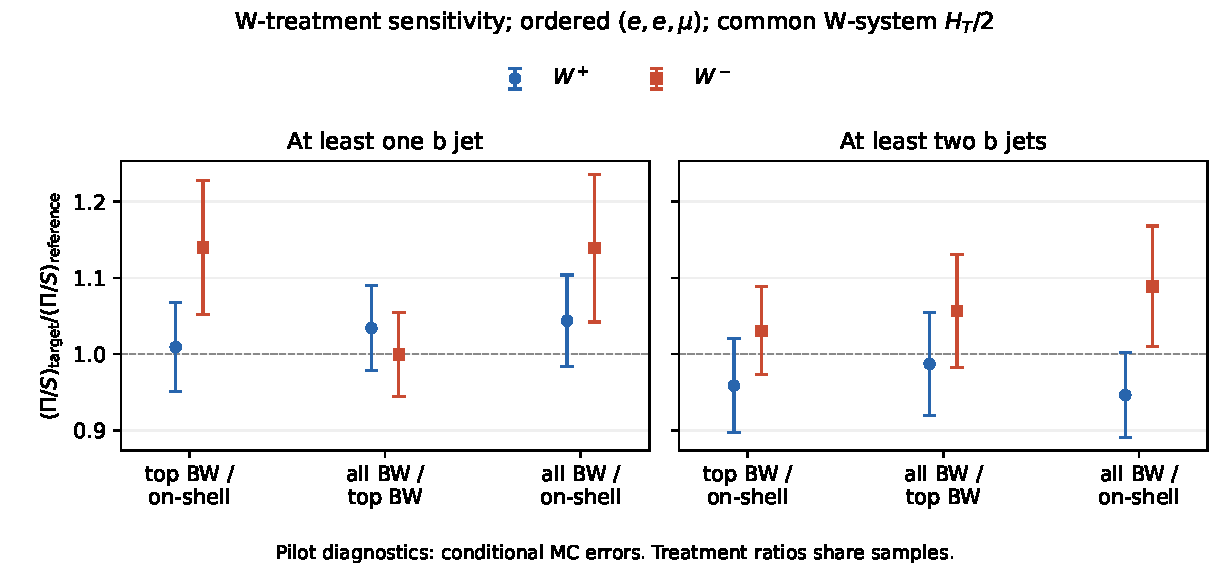
\includegraphics[width=\linewidth]{../figures/w_treatment_pilot_width_mass_v2.pdf}
\caption{W-treatment changes of the product/strict ratio for the single
ordered $e,e,\mu$ assignment in both charges. Bars are conditional MC
errors, and the three treatment ratios share samples. These pilot
diagnostics use matched widths and common dynamic production scales;
they are not full-flavour predictions or a convergence certification.}
\label{fig:wtreatmentpilot}
\end{figure}

The massive-decay companions retain massless five-flavour production:
88 source files for production, flavour data and virtuals, and the production-owned FKS
records match the massless export exactly. The massive parameter-card
round trip and all 120 pre-integration pole checks pass. The first massive
strict-sum pilot completed, but its product companion stopped on a local
Born-snapshot alignment check. The cause was a different daughter ordering
in the canonical tree and the massive NLO context. An explicit-identity
permutation fix passes 2400 deterministic Born-map checks, and fresh
on-shell and all-BW massive S/Pi pairs pass the full pilot audits.
The massive/massless double ratio of $\Pi/S$, formed before scale/PDF
reduction with four independent sample/stratum ensembles, is
$1.038\pm0.053$ ($1.007\pm0.050$) in the on-shell one-b (two-b) selection
and $0.921\pm0.053$ ($0.953\pm0.067$) for all BW. These conditional MC
errors do not resolve a mass dependence at the specified precision.
The completed W$^-$ companions give double ratios
$1.146\pm0.090$ ($1.109\pm0.064$) for the on-shell one-b (two-b)
selection and $0.976\pm0.059$ ($0.955\pm0.070$) for all BW.
These single-assignment results also do not resolve a mass dependence.
Independent-retraining convergence, small-mass continuity and the main
flavour-summed mass/width-scheme comparison remain open.

\paragraph{Generated narrow-W limit.}
The 21 massless-decay LO/S/$\Pi$ tests now contain an on-shell reference
and top-BW/all-BW samples at
$\epsilon=\Gamma_W/\Gamma_W^{\rm ref}=1,0.2,0.05$ for each prescription.
All use the common fixed scale $m_t+M_W/2=212.6925\GeV$ for production,
both decay numerators and the reference coupling in the top widths.
Weak couplings remain fixed while the matched top widths are recalculated.
The finite comparison is $\epsilon^3\sigma_{\rm BW}/\sigma_{\rm on\ shell}$:
each selected leptonic W density supplies one inverse power of $\epsilon$.
This factor is applied once to the reported cross sections, with no change
to the generated event weights and no additional branching factors.

At $\epsilon=0.05$, the LO two-b ratios are
$1.0028\pm0.0067$ (top BW) and $1.0032\pm0.0063$ (all BW).
For $\Pi$ they are $1.023\pm0.038$ and $1.022\pm0.040$;
for S they are $0.847\pm0.121$ and $0.872\pm0.124$.
These are conditional joint MC errors from independent run/beam strata,
with the common on-shell reference propagated to all width points.
The S comparison is limited particularly by the imprecise on-shell
fiducial reference. It does not establish percent-level NLO continuity.
Across six coarsened spectra at the narrowest width, the largest absolute
normalized-bin residuals are 2.13, 2.74 and 2.05 conditional MC errors
for LO, S and $\Pi$, respectively. These correlated bin residuals are
diagnostics, not a global goodness-of-fit test. The coarse bins retain
the original range and are summed before normalization to the matching
fiducial rate. Unmeasured continuous overflows are not folded into them.
All 81 scale and 101 PDF coordinates are retained in the comparison arrays.

\begin{figure}[ht]
\centering
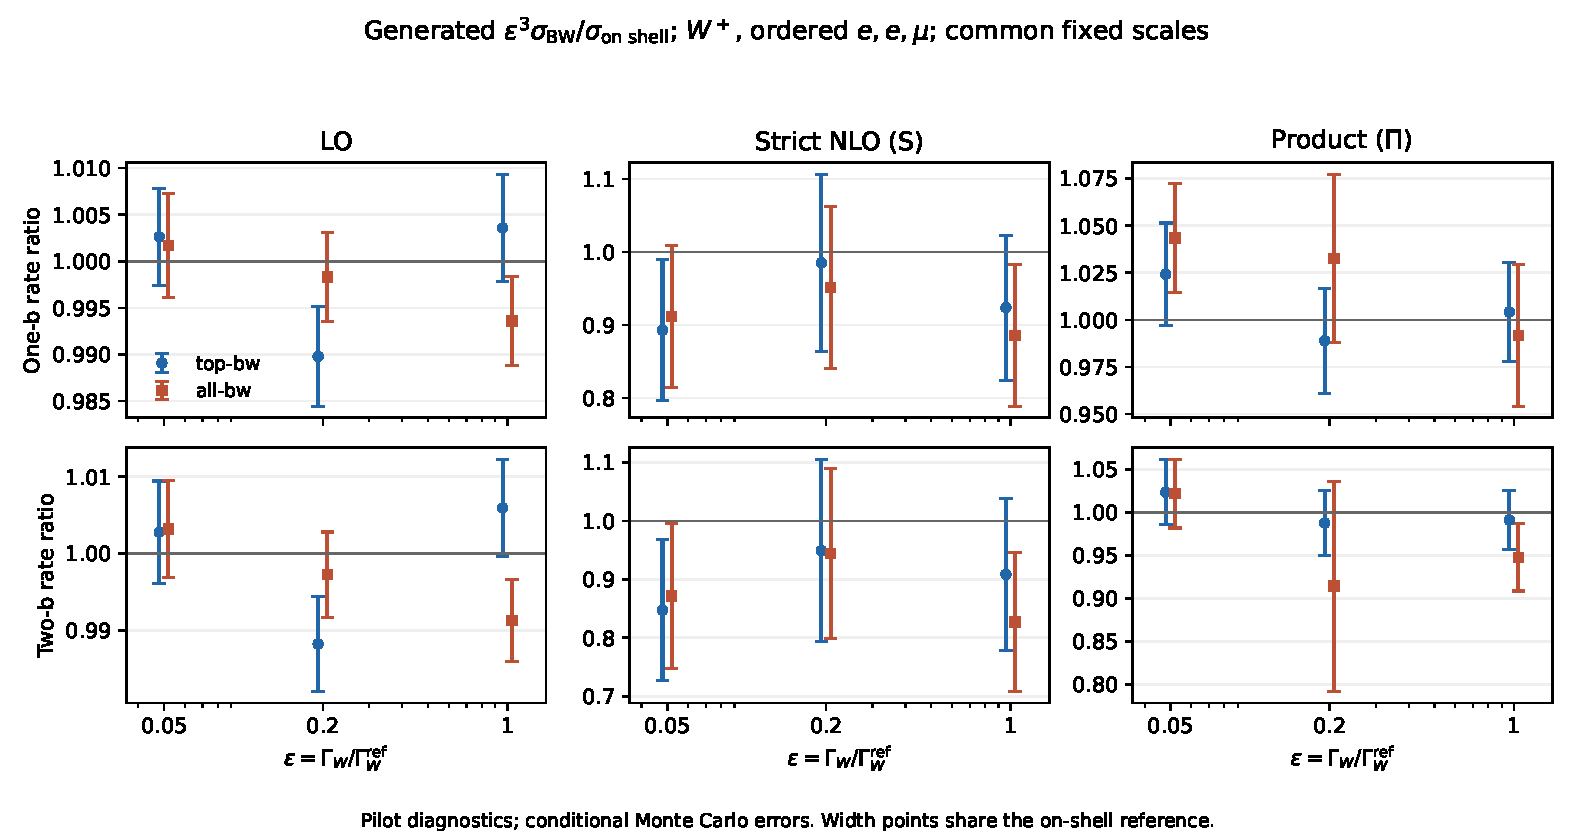
\includegraphics[width=\linewidth]{../figures/generated_narrow_w.pdf}
\caption{Generated narrow-W diagnostics for the single ordered W+
$e,e,\mu$ assignment at common fixed scales. Vertical bars show conditional
MC errors; points at different widths share the on-shell reference.
Horizontal offsets separate the two W treatments. Each panel has its own
vertical scale. These pilot results are not full-flavour predictions or a
percent-level NLO convergence certification.}
\label{fig:narrowW}
\end{figure}

Full-flavour and NLO varied-weight normalization, direct scale
reweighting checks, small-mass validation and integration convergence
remain open. Matched ttW and dilepton-ttbar reference pilots have completed;
their subsequent direct-scale and absolute-normalization tests are in progress.
